\section{Experiments}
\subsection{Experimental setup}
%%===data===%%
We train and evaluate our models on the ShapeNet\cite{shapenetdata}. Specifically, we use the ShapeNetCore55.v2 which contains over 50k of
manually created and cleaned 3D CAD models in 55 category.
The images for training
and testing are rendered in random angles to provide synthetic training data for the model. In total,
51,856 shape models are covered. For the training/validation/testing split, we follow the CSV file provided by the ShapeNet website and resulted in 36,622/5,110/10,124 shapes. The 3D CAD objects are
stored as meshes, we re-sample the meshes into point sets. In order to capture only the shape surface, we uses the code from \cite{Wang-2017-OCNN} and execute ``virtual scan" for the re-sampling.
\subsection{Comparing to state-of-the-art}
In this subsection, we compare our approach with point set generation network (PSGN)\cite{PSGN} 
with (we use ball-pivoting\cite{ballpivot} to generate mesh for the point set).
\begin{figure*}[htbp]
	\centering
	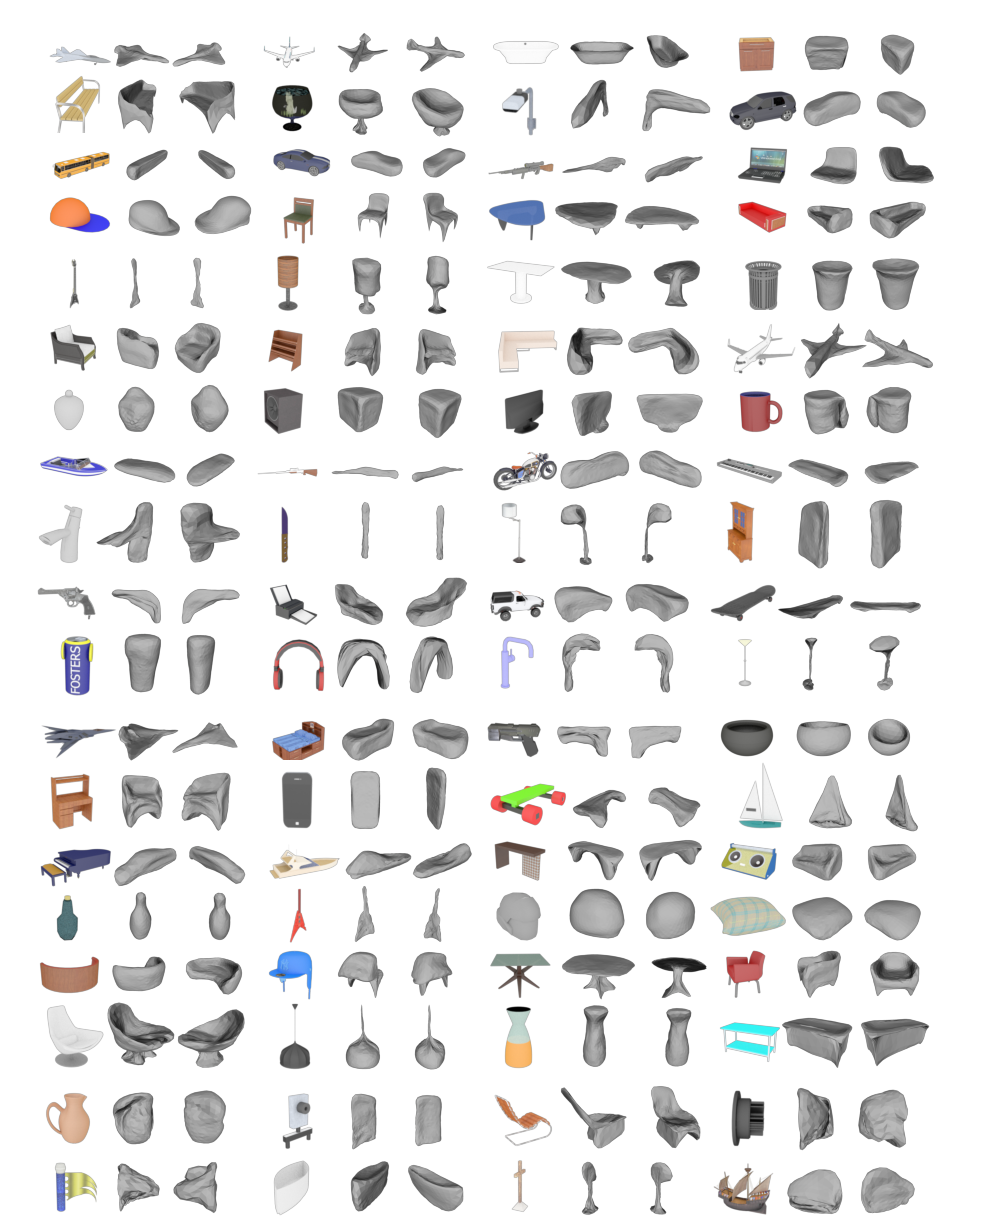
\includegraphics[width=\linewidth]{img/res/res}
	\caption{The comparison of visual results}
	\label{fig:res}
\end{figure*}
 

\subsection{Ablation study}
\begin{table*}
	\caption{Ablation study with respect to different components}
	\label{tab:ablation}
	\centering
	\begin{tabular}{c | c c c c c}
		Models &  Full Model  & -Initialization & -Laplation smooth & -Edge Length Regularization & -Norm Loss \\
		\hline
		Chamfer      & 0.297 & 0.424 & 0.394 & 0.405  & 0.390\\
		EMD			 & 0.834 & 1.524 & 1.369 & 4.195  & 1.415
	\end{tabular}
\end{table*}
\noindent\textbf{Laplacian smooth}

\noindent\textbf{Initialization}

\noindent\textbf{Edge Length Regularization}

\noindent\textbf{Number of \textit{K}-neighbor PointNet}
\begin{table}
	\caption{Ablation study with respect to number of \textit{K}-neighbor PointNet}
	\label{tab:pointnet}
	\centering
	\begin{tabular}{c | c c c c}
		Number of \textit{K}-neighbor PointNet &  2 & 3 & 4 & 5 \\
		\hline
		Chamfer      & 0.425 &  0.411 & 0.297 & 0.313 \\
		EMD			 & 1.304 &  1.360 & 0.834 & 1.067
	\end{tabular}
\end{table}
\subsection{Semantic and sampling variation}
add semantic random vector to ParamNet and PSGN\cite{PSGN}